\documentclass[aps,twocolumn,twoside,secnumarabic,balancelastpage,amsmath,amssymb,nofootinbib,hyperref=pdftex]{revtex4}

%\usepackage{lgrind}        
\usepackage{chapterbib}    
\usepackage{color}         
\usepackage{graphics}      
\usepackage[pdftex]{graphicx}      
\usepackage{longtable}     
\usepackage{epsf}          
\usepackage{bm}           
\usepackage{verbatim}
\usepackage{gensymb}
%\usepackage{asymptote}     
%\usepackage{thumbpdf}
%\usepackage{xcolor}
\usepackage[colorlinks=true, urlcolor=green]{hyperref}  
                                       
\usepackage{array,tabularx}
 
\addtolength\topmargin{-.5\topmargin} 

\newenvironment{EqParameters}[1][]
  {#1 \begin{tabular}[t]{>{$}l<{$} @{${}={}$} l}}
  {\end{tabular}\\[\belowdisplayskip]}

\begin{document}
\title{Ultraviolet and Visible Spectroscopy for Fluids}
\author         {Eduardo L. Bemelmans}
\email          {eduardo.bemelmans@student.pxl.be}
\homepage{https://github.com/PXL-Embedded-AI/repo/issues/24}
\date{\today}
\affiliation{PXL University of applied sciences and arts, Department PXL-Digital: Electronics-ICT}


\begin{abstract}



\end{abstract}

\maketitle

%%%%%%%%%%%%%%%%%%%%%%%%%%%%%%%%%%%%%%%%%%%%%%%%%%%%%%%%%%%%%%%%%%

\section{Introduction}
UV and Vis spectroscopy allows determination of different organic compounds. In particular, fluids absorb light in the UV or visible range. The spectrum of every fluid, like any organic compound, is unique. Within the chemical process technology it is desired to be able to detect a difference in fluids. A UV-Vis spectroscopy measurement apparatus could provide a solution to automate the process of determining fluid deltas. Combined with an embedded AI system, predictions based on the deltas can be made. This document discusses the theory and implementation of UV-Vis spectroscopy for fluids.

\section{Theory}
\subsection{Principle}

The following equation is known as the grating equation\cite{geqs}: %Eq.~\ref{eq:gratingEquation1}
\begin{equation}
   d(\sin{\alpha}+\sin{\beta})=m\lambda 
   \label{eq:gratingEquation1}
\end{equation}
Where:
\begin{EqParameters}
d    &  spacing between the slits (the grating spacing) \\
\alpha &  the incident angle \\
\beta &  the diffraction angle \\
m    &  the order of the spectrum \\
\lambda & the wavelength \\
\end{EqParameters}

The number of slits per unit of length $N$ is usually specified for diffraction gratings.
Since
\begin{equation}
   d = \frac{1}{N}
   \label{eq:grSp1}
\end{equation}

Eq.~\ref{eq:gratingEquation1} can be rewritten in terms of the number of slits or lines per unit length:

\begin{equation}
   \sin{\alpha}+\sin{\beta}=Nm\lambda 
   \label{eq:gratingEquationwrN}
\end{equation}

The angle $\alpha$ is the angle between the incident light and the normal of the grating, and $\beta$ is the angle between the diffracted light and the normal of the grating. Notice the plus sign instead of minus in the equation. The incident angle is measured counter-clockwise from the grating normal and the diffraction angle is measured clockwise from the grating normal. This is a sign convention for transmission gratings. The equation governs the angular locations of the diffracted light of wavelength $\lambda$. In our research project, transmission gratings are used to construct a simple test model as shown in Fig.~\ref{fig:tr_gr}.

\begin{figure}[htb]
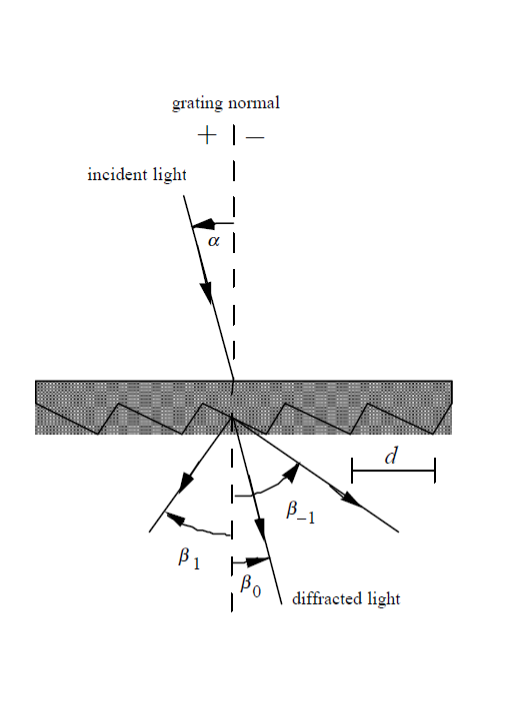
\includegraphics[width=5cm, height=8cm]{tr_gr_angles}
\caption{Diffraction by a plane transmission grating. Adapted from \cite{Palmer2005}.
\label{fig:tr_gr}}
\end{figure}

\begin{comment}
To simplify the construction of the testmodel, the incident light beam must be parallel to the grating normal. Hence, defining $\theta = \beta_{-1}$, Eq.~\ref{eq:gratingEquation1} reduces to:

\begin{equation}
   d\sin{\theta}=m\lambda 
   \label{eq:gratingEquation2}
\end{equation}
\end{comment}

This implies that the the camera must be placed at a specific angle so that it can capture the spectrum of the first order ($m=1$). According to \cite{mchr} (see: mountings), aligning elements can be used to refine the operation of the spectroscopy meter. Fig.~\ref{fig:sp_m} shows the setup for a monochromator. The alignment elements used in this setup can also be applied to our spectrometer prototype. From the entrance slit (1), the light diverges to a collimating mirror (2). This mirror reforms the diverging incident light beam to a parallel light beam. The diffraction grating (3) is a reflective grating which reflects and disperses the light beam into different colors (and at an angle, governed by Eq.~\ref{eq:gratingEquation1}). Since we want to capture the first order spectrum, a camera substitutes the camera mirror (4) in our project. In case a more advanced prototype is required, this setup must be considered. A video \cite{spwo} shows the operation of this setup.

\begin{figure}[htb]
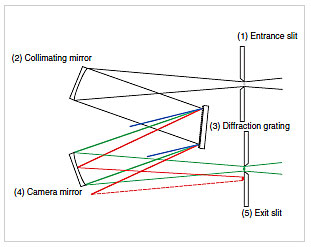
\includegraphics[width=7cm, height=5cm]{mountings.jpg}
\caption{Aligning elements for a monochromator. Adapted from \cite{mchr}.
\label{fig:sp_m}}
\end{figure}


\subsection{Implementation}
Fluids can absorb light in the UV and the full (adjacent) visible spectral region. Therefore, the wavelength ranges from around 200 to 740nm. This is a complication as a source lamp which is bright, continuous, and stable across this range is required \cite{lssp}. For the test model, a tungsten halogen lamp can be used. This lamp however, only covers the visible spectral region. The prototype should be armed with a more advanced source light system as shown in Fig.~\ref{fig:sw-lssp}. According to \cite{lssp}, the deuterium lamp is a continuous spectrum light source which is stable in the UV region.  

\begin{figure}[htb]
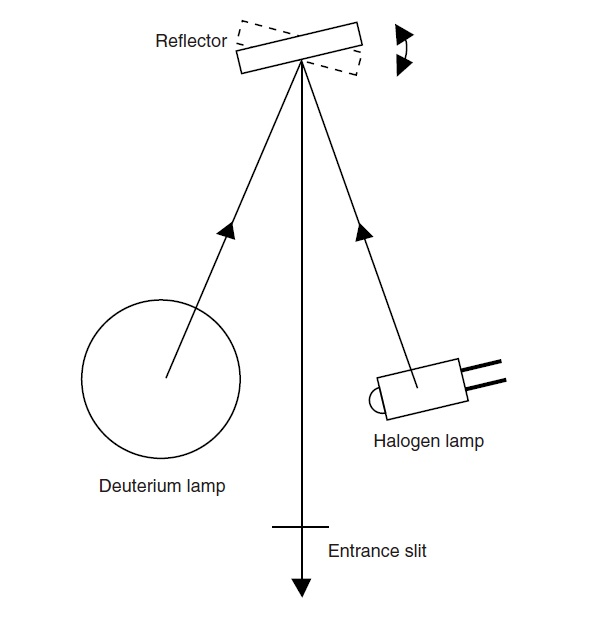
\includegraphics[width=6cm, height=5cm]{sw-lssp.jpg}
\caption{Switching light sources. Adapted from \cite{lssp}.
\label{fig:sw-lssp}}
\end{figure}

\section{Analysis and results}
To simplify the construction of the test model, the angle of incidence is zero. Table~\ref{tab:table1} shows the diffraction angle with respect to the wavelength for the testmodel with a diffraction grating having 600 lines/mm. Table~\ref{tab:table2} shows the same parameters, however the diffraction grating has 1000 lines/mm. Table~\ref{tab:table3} again shows the same parameters but in this case, the angle of incidence is $-20\degree$ and the diffraction grating has 600 lines/mm. All tables show the data for the first order spectrum. 

The results for $\beta$ from table~\ref{tab:table1} indicate that the first order spectrum is spread over $\approx19.50\degree$, which is well within the FOV of the camera. Table~\ref{tab:table2} and~\ref{tab:table3} show that, when $N$ or $\alpha$ is altered, the spectrum spreads over a wider angle. When $\alpha=0$, and $N=1000$ the spectrum spreads over $\approx36.20\degree$, whereas if $\alpha=-20\degree$, and $N=600$, the spectrum spreads over $22.30\degree$.

\begin{table}[htb]
\caption{\label{tab:table1}Diffraction angle $\beta$, where $\alpha=0$\degree, $m=1$, and $N=600$ lines per millimeter.}
\begin{ruledtabular}
\begin{tabular}{ccc}
&$\lambda$ (nm) &$\beta$ (\degree)\\
\hline
UV      & 200 & 6.89  \\
Violet  & 380 & 13.89 \\
Blue    & 435 & 15.13 \\
Cyan    & 500 & 17.46 \\
Green   & 520 & 18.18 \\
Yellow  & 565 & 19.82 \\
Orange  & 590 & 20.73 \\
Red     & 625 & 22.02 \\
        & 740 & 26.36 \\
\end{tabular}
\end{ruledtabular}
%\footnotetext[1]{}
\end{table}
\begin{table}[htb]
\caption{\label{tab:table2}Diffraction angle $\beta$, where $\alpha=0$\degree, $m=1$, and $N=1000$ lines per millimeter.}
\begin{ruledtabular}
\begin{tabular}{ccc}
&$\lambda$ (nm) &$\beta$ (\degree)\\
\hline
UV      & 200 & 11.54 \\
Violet  & 380 & 22.33 \\
Blue    & 435 & 25.79 \\
Cyan    & 500 & 30 \\
Green   & 520 & 31.33 \\
Yellow  & 565 & 34.40 \\
Orange  & 590 & 36.16 \\
Red     & 625 & 38.68 \\
        & 740 & 47.73 \\
\end{tabular}
\end{ruledtabular}
%\footnotetext[1]{}
\end{table}
\begin{table}[htb]
\caption{\label{tab:table3}Diffraction angle $\beta$, where $\alpha=-20$\degree, $m=1$, and $N=600$ lines per millimeter.}
\begin{ruledtabular}
\begin{tabular}{ccc}
&$\lambda$ (nm) &$\beta$ (\degree)\\
\hline
UV      & 200 & 27.52 \\
Violet  & 380 & 34.75 \\
Blue    & 435 & 37.09 \\
Cyan    & 500 & 39.94 \\
Green   & 520 & 40.85 \\
Yellow  & 565 & 42.92 \\
Orange  & 590 & 44.11 \\
Red     & 625 & 45.81 \\
        & 740 & 51.82 \\
\end{tabular}
\end{ruledtabular}
%\footnotetext[1]{}
\end{table}

\section{Conclusion}


%bibliograhy.
\section{Bibliography notes}

\bibliography{spectro-bib}

\end{document}
